\section{Views}\label{c:views}

As \textit{Views} variam consoante o tipo de utilizador tendo, assim, em conta de quem é proveniente o pedido (garantido através do \texttt{type} guardado na sessão). Para além disso, o sistema recorre ao uso de \texttt{jquery} de forma a tornar as páginas web mais funcionais, tais como o uso de filtros para filtrar o conteúdo a mostrar consoante o input do utilizador.

Por outro lado, por forma a mostrar os erros e/ou os sucessos por parte do utilizador, o sistema usa a package \texttt{connect-flash} como \texttt{middleware} que permite gravar nas sessões valores a apresentar. No fundo, isto permite que seja guardado o erro/sucesso a transmitir, ocorra o redirecionamento para uma página e, por fim, apresentar o erro/sucesso ao utilizador.

Na pasta \texttt{View} podemos encontrar sete sub-pastas correspondentes às \textit{views} dos artigos, das \textit{entries} (biblioteca de suporte), dos eventos, dos menus, das peças musicais, das estatísticas e, por fim, dos utilizadores. Para além das pastas, há ainda três ficheiros: a \textit{view} dos erros, o \textit{layout} básico, e um segundo \textit{layout} que dá \textit{extend} do primeiro.

\begin{framed}
\begin{lstlisting}[language=pug]
    doctype html
    html
        head
            title iBanda
            link(rel='stylesheet', href='/stylesheets/w3.css')
            link(rel='shortcut icon' href='images/favicon.ico' type='image/icon')
            script(src="/javascripts/jquery-3.3.1.min.js")
            script.
                var url = "!{url}"
            block scripts
        body
            block content
\end{lstlisting}
\end{framed}

\begin{center}
\textit{Ficheiro} \texttt{layout.pug} \textit{da pasta} \texttt{Views} \textit{correspondente ao layout geral da aplicação.}
\end{center}

\begin{framed}
\begin{lstlisting}[language=pug]
extends layout

block content
    .w3-container
        .w3-card-4
            header.w3-container.w3-grey
                block header
            .w3-container
                block body
            footer.w3-container.w3-grey
                address iBanda
\end{lstlisting}
\end{framed}

\begin{center}
\textit{Ficheiro} \texttt{layout2.pug} \textit{da pasta} \texttt{Views} \textit{correspondente ao layout extendido da aplicação.}
\end{center}


A nível da interface, podemos ver nas figuras que se seguem alguns exemplos relativos às vistas disponíveis para um administrador.

A figura \ref{fig:menuObras} ilustra um dos menus disponíveis, nomeadamente o menu das obras musicais no qual este pode consultar as várias obras disponíveis.

\begin{figure}[H]
\begin{center}
    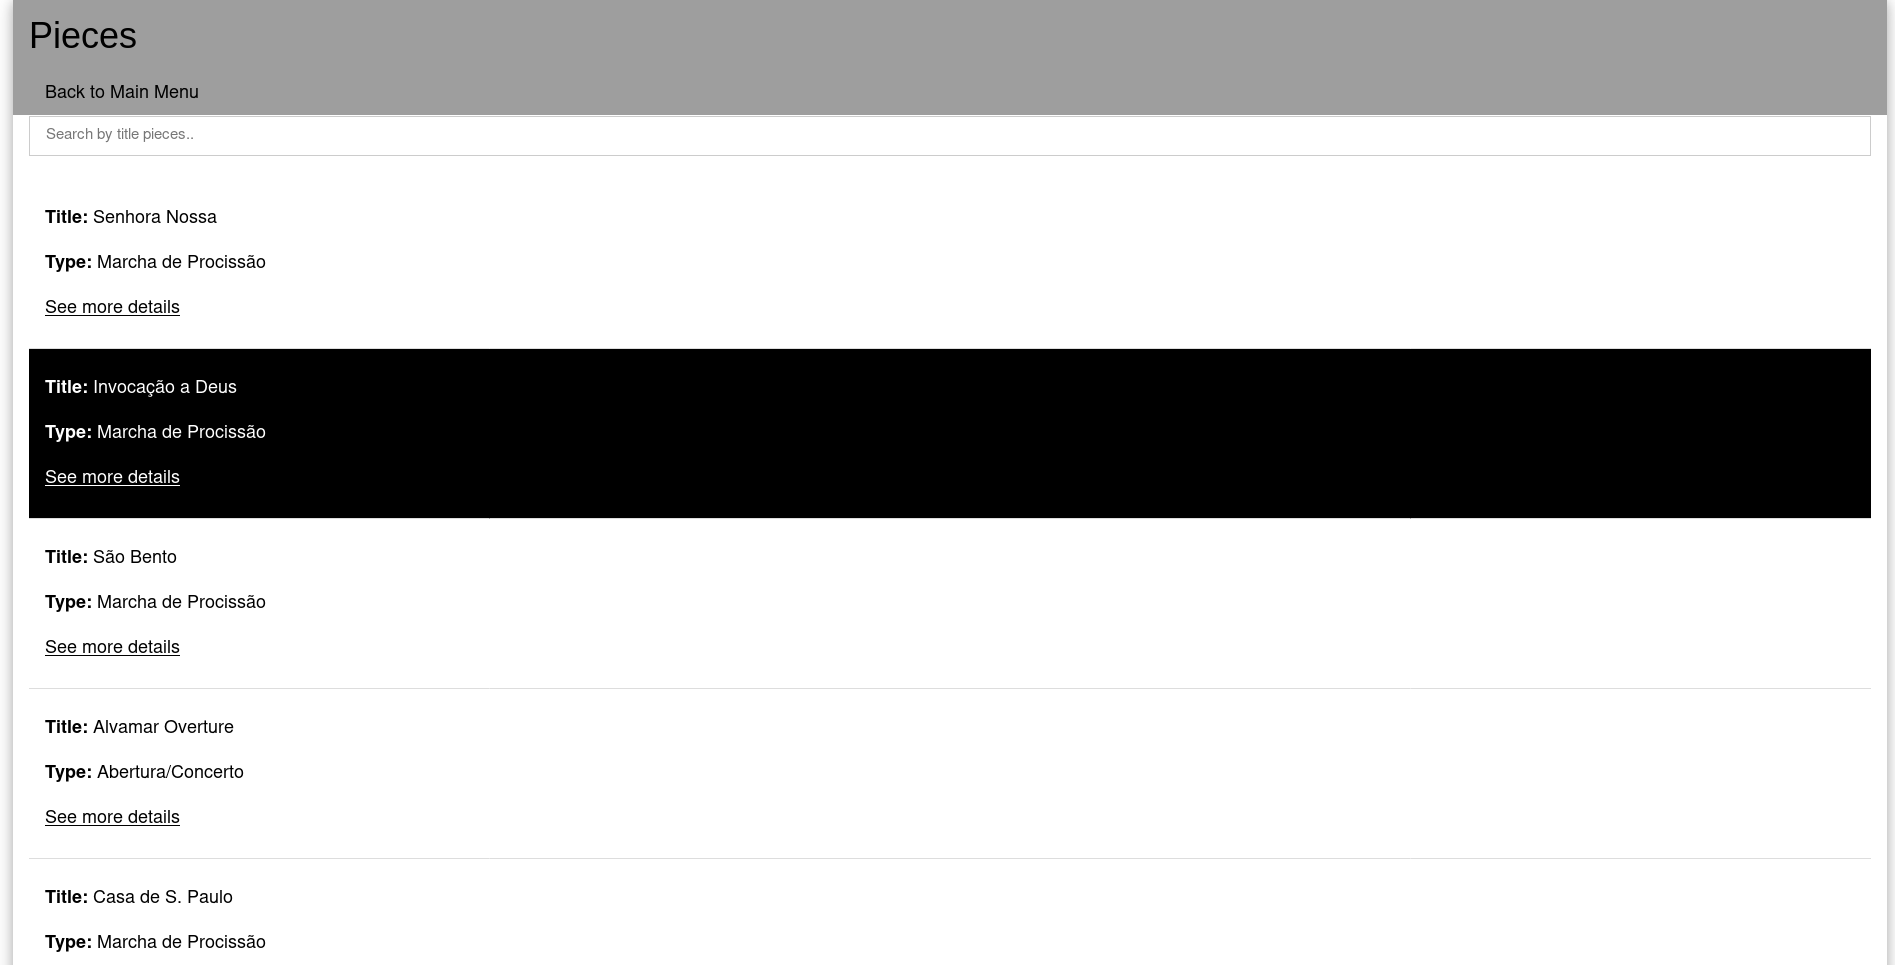
\includegraphics[width = 0.9\textwidth, keepaspectratio]{imgs/piecesMenu.png}
    \caption{\textit{Menu das obras musicais ("Pieces") disponível para um utilizador pertencente à categoria de "administrador".}}
    \label{fig:menuObras}
\end{center}
\end{figure}

Assumindo que um administrador pretende consultar uma obra específica do menu acima mencionado, a vista resultante seria como a exemplificada na figura \ref{fig:umaObra}. 

\begin{figure}[H]
\begin{center}
    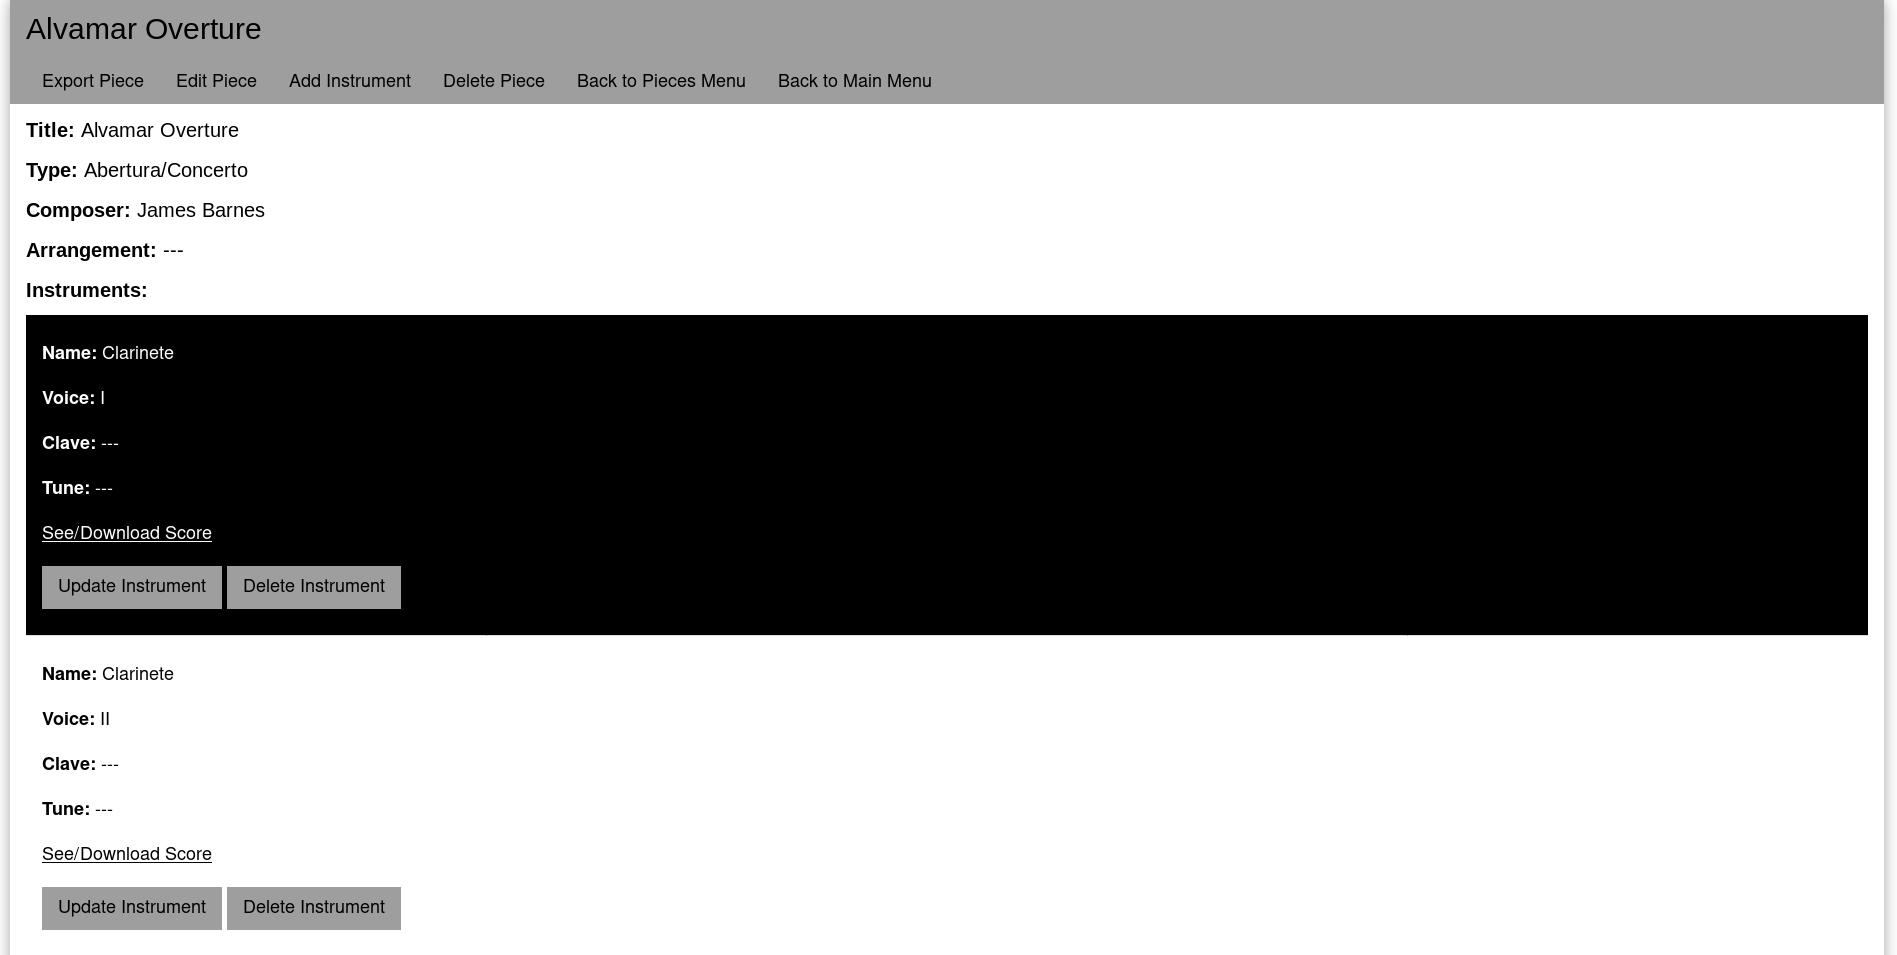
\includegraphics[width = 0.8\textwidth, keepaspectratio]{imgs/onePiece.png}
    \caption{\textit{Exemplo de uma obra disponível para um utilizador pertencente à categoria de "administrador".}}
    \label{fig:umaObra}
\end{center}
\end{figure}

Por fim, caso um administrador pretenda consultar estatísticas relativas às aplicação, como por exemplo \textit{"User with most downloads"} e \textit{"Piece with most views"}, ser-lhe-á apresentada uma vista como a da figura \ref{fig:statsMenu}.

\begin{figure}[H]
\begin{center}
    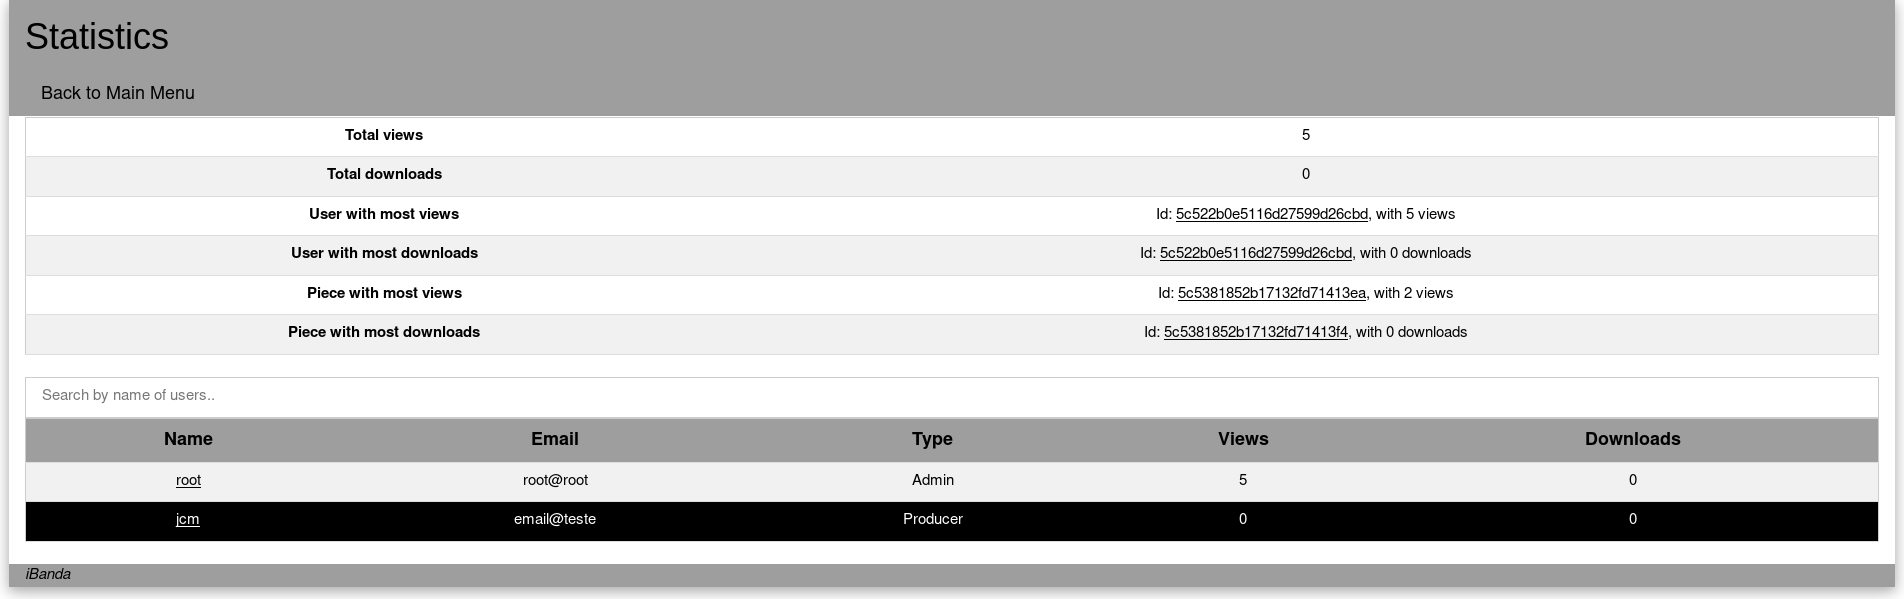
\includegraphics[width = 0.8\textwidth, keepaspectratio]{imgs/statisticsMenu.png}
    \caption{\textit{Menu das estatísticas disponível para um utilizador pertencente à categoria de "administrador".}}
    \label{fig:statsMenu}
\end{center}
\end{figure}